\PassOptionsToPackage{unicode=true}{hyperref} % options for packages loaded elsewhere
\PassOptionsToPackage{hyphens}{url}
%
\documentclass[]{article}
\usepackage{lmodern}
\usepackage{amssymb,amsmath}
\usepackage{ifxetex,ifluatex}
\usepackage{fixltx2e} % provides \textsubscript
\ifnum 0\ifxetex 1\fi\ifluatex 1\fi=0 % if pdftex
  \usepackage[T1]{fontenc}
  \usepackage[utf8]{inputenc}
  \usepackage{textcomp} % provides euro and other symbols
\else % if luatex or xelatex
  \usepackage{unicode-math}
  \defaultfontfeatures{Ligatures=TeX,Scale=MatchLowercase}
\fi
% use upquote if available, for straight quotes in verbatim environments
\IfFileExists{upquote.sty}{\usepackage{upquote}}{}
% use microtype if available
\IfFileExists{microtype.sty}{%
\usepackage[]{microtype}
\UseMicrotypeSet[protrusion]{basicmath} % disable protrusion for tt fonts
}{}
\IfFileExists{parskip.sty}{%
\usepackage{parskip}
}{% else
\setlength{\parindent}{0pt}
\setlength{\parskip}{6pt plus 2pt minus 1pt}
}
\usepackage{hyperref}
\hypersetup{
            pdfborder={0 0 0},
            breaklinks=true}
\urlstyle{same}  % don't use monospace font for urls
\usepackage[margin=1in]{geometry}
\usepackage{graphicx,grffile}
\makeatletter
\def\maxwidth{\ifdim\Gin@nat@width>\linewidth\linewidth\else\Gin@nat@width\fi}
\def\maxheight{\ifdim\Gin@nat@height>\textheight\textheight\else\Gin@nat@height\fi}
\makeatother
% Scale images if necessary, so that they will not overflow the page
% margins by default, and it is still possible to overwrite the defaults
% using explicit options in \includegraphics[width, height, ...]{}
\setkeys{Gin}{width=\maxwidth,height=\maxheight,keepaspectratio}
\setlength{\emergencystretch}{3em}  % prevent overfull lines
\providecommand{\tightlist}{%
  \setlength{\itemsep}{0pt}\setlength{\parskip}{0pt}}
\setcounter{secnumdepth}{0}
% Redefines (sub)paragraphs to behave more like sections
\ifx\paragraph\undefined\else
\let\oldparagraph\paragraph
\renewcommand{\paragraph}[1]{\oldparagraph{#1}\mbox{}}
\fi
\ifx\subparagraph\undefined\else
\let\oldsubparagraph\subparagraph
\renewcommand{\subparagraph}[1]{\oldsubparagraph{#1}\mbox{}}
\fi

% set default figure placement to htbp
\makeatletter
\def\fps@figure{htbp}
\makeatother

\usepackage{ctex}
\setmainfont{STHeitiSC-Medium}
\setCJKmainfont{STHeitiSC-Medium}
\usepackage{xcolor}
\usepackage{fancyhdr}
\pagestyle{plain}
\usepackage{sectsty}
\definecolor{glaucous}{rgb}{0.38, 0.51, 0.71}
\definecolor{lavenderblush}{rgb}{1.0, 0.94, 0.96}
\definecolor{grey}{RGB}{96, 96, 96}
\usepackage{enumitem}% http://ctan.org/pkg/enumitem
\usepackage[empty]{fullpage}% http://ctan.org/pkg/fullpage
\usepackage{color}% http://ctan.org/pkg/color
\usepackage{hyperref}% http://ctan.org/pkg/hyperref
\usepackage{geometry}
\geometry{papersize={15.5cm,50cm},left=0.5cm,right=0.5cm,top=0.3cm,bottom=0.3cm}
\usepackage{blindtext}
\usepackage[center]{caption}
\usepackage[font=Large]{caption}
\usepackage{subfigure}
\usepackage{float}
\usepackage{graphicx}
\usepackage{booktabs}
\usepackage[justification=centering]{caption}
\usepackage{threeparttable}
\usepackage{longtable}
\usepackage{array}
\usepackage{multirow}
\usepackage{wrapfig}
\usepackage{float}
\usepackage{colortbl}
\usepackage{pdflscape}
\usepackage{tabu}
\usepackage{threeparttable}
\usepackage{threeparttablex}
\usepackage[normalem]{ulem}
\usepackage{makecell}
\usepackage{xcolor}
\linespread{1.85}
\setlength{\parskip}{1em}
\setlength{\footskip}{20pt}
\usepackage{booktabs}
\usepackage{longtable}
\usepackage{array}
\usepackage{multirow}
\usepackage{wrapfig}
\usepackage{float}
\usepackage{colortbl}
\usepackage{pdflscape}
\usepackage{tabu}
\usepackage{threeparttable}
\usepackage{threeparttablex}
\usepackage[normalem]{ulem}
\usepackage{makecell}
\usepackage{xcolor}

\author{}
\date{\vspace{-2.5em}}

\begin{document}

\captionsetup[figure]{name={图},labelsep=space}
\captionsetup[table]{name={表},labelsep=space} 
\fontsize{22}{22}
\selectfont
\vspace{-10truemm}

\newcommand{\resheading}[1]{%
  \noindent\fcolorbox{lavenderblush}{lavenderblush}{\makebox[\dimexpr\textwidth-2\fboxsep-2\fboxrule][c]{\textbf{~#1}}}%
}

\newcommand\fnote[1]{\captionsetup{font=large}\caption*{#1}}

\begin{center}

\includegraphics[height=2cm]{./input/logo2.png} 
\end{center}

\begin{center}
\fontsize{45}{45}
\textcolor{glaucous}{\textbf{新冠早报}}
\end{center}

\begin{center}
\fontsize{22}{22}
{\textcolor{glaucous}{\textbf{第84期 \space 7月16日}}}
\end{center}

\vspace{2mm}
\begin{center}

\includegraphics[height=2cm]{./input/title1.png} 
\end{center}

\begin{center}
编者 : 张三
\end{center}

\vspace{-5mm}

\begin{huge}{\textcolor{glaucous}{\textbf{国际}}}\end{huge}

\vspace{-3mm}

\begin{center}
\textcolor{glaucous}{华尔街日报(The Wall Street Journal)}\\美国、沙特和俄罗斯牵头达成创纪录的石油减产协议

\end{center}

由于新冠危机导致石油需求下降,加上沙特与俄罗斯之间产生争执,油价受到重创。有鉴于此,当地时间4月12日,沙特、俄罗斯和美国同意牵头一个多国联盟进行大规模石油减产。按照协议,23个国家承诺每日总计减产970万桶石油,减产幅度达到创纪录水平。

\begin{center}
\textcolor{glaucous}{有线电视新闻网(CNN)}\\新冠病毒模型表示,今天是美国单日死亡的高峰
\end{center}

当地时间4月13日,据白宫引用的一种新冠病毒模型表示,今天是美国每日死亡的高峰日。根据华盛顿大学健康指标与评估研究所的模型,今天预计将有2150例死亡,并且死亡人数有望继续下降。

\begin{center}
\textcolor{glaucous}{华盛顿邮报(Washington Post)}\\韩国将向美国出口首批60万个新冠病毒测试盒
\end{center}

当地时间4月13日,韩国政府官员透露,韩国计划于本周二向美国运送60万个新冠病毒测验试剂盒,这是上月韩国总统文在寅收到美国总统特朗普电话求援后,韩国向美国运送的首批此类物资。

\begin{center}
\textcolor{glaucous}{纽约时报(New York Times)}\\法国和英国将延长封锁令至5月
\end{center}

当地时间4月13日晚,法国总统马克龙宣布,将法国全境执行的封锁令延长至5月11日,从这一天开始,法国将对所有出现新冠肺炎疑似症状的病患进行病毒检测,所有民众都将能买到口罩。同一天,由于没有迹象表明疫情在好转,英国首相约翰逊也表示将原定于4月13日结束的全境封锁令延长至5月

\begin{center}
\textcolor{glaucous}{华盛顿邮报(Washington Post)}\\西班牙疫情趋缓,部分产业开始复工
\end{center}

当地时间4月13日,西班牙新冠病毒的新增死亡病例重返下滑趋势,新增确诊也减至3周以来最少。该国制造业员工今天重返工作岗位,警察与红十字会志愿者在火车站向返工人士分发口罩。

\vspace{5mm}

\begin{huge}{\textcolor{glaucous}{\textbf {国内}}}\end{huge}

\vspace{-3mm}

\begin{center}
\textcolor{glaucous}{中新网}\\聚集性病例“抬头” ,中国本土新增确诊病例创近一月来新高
\end{center}

北京时间4月12日,官方数据显示,中国内地新增境外输入确诊病例98例,再创单日增长新高;本土新增确诊病例10例,为3月11日以来单日最高,且多为聚集性病例。中国疫情防控外防输入、内防反弹形势严峻。

\begin{center}
\textcolor{glaucous}{BBC中文}\\非洲裔人士在中国广州“被歧视” 引发外交风波
\end{center}

近日,数百名在中国广州居住的非洲裔居民,在没有被确诊新冠肺炎下,被赶出家门、强制检疫和没收护照。非洲联盟及多个非洲国家发声关注广州非裔人士的处境,强烈谴责有人歧视和不人道对待当地非洲人。中国外交部表示,实施抗疫措施时出现``一些情况和误解'',中方高度重视,将``敦促相关方面改善工作机制和方法'',强调中国和非洲会相互支持、携手抗疫。

\vspace{15mm}

\begin{center}

\includegraphics[height=2cm]{./input/title3.png} 
\end{center}
\vspace{-7mm}

\vspace{5mm}

\begin{center}
\textcolor{glaucous}{\Huge 后疫情时代的高考——“在最可怕的时刻怀抱希望”
}
\end{center}

\vspace{-3mm}

\begin{center}
作者: 张三
\end{center}

\(\quad\)高考结束的那天,你做了什么?这样一个话题,年年都会在炎热的6月登上全国社交媒体的热搜。它经久不息,似乎老套至极。然而每一次被这样的话题刷屏,我好像都能短暂的与多年以前的青春、高考再次面对面。\(\quad\)而2020作为如此特殊的一年,高考自然也格外不同寻常。受疫情影响,2020年普通高等学校招生全国统一考试(简称:2020年全国高考)的考试时间,定为2020年7月7日至2020年7月8日\(^1\)。(北京地区例外:高考时间为7月7日到7月10日。)而今年的高考报名人数也达到了1071万余人\(^2\),比2019年度增加约40万考生\(^2\)。今年全国将设考点7000余个、考场40万个\(^4\)。而今年的高考成绩,将于2020年7月26日17时公布\(^5\)。
而部分地区,例如安徽歙县,受今年我国南方大面积降雨的影响,出现了考试延迟\(^6\)。

\(\quad\)有关高考作文,高考数学题目的话题再一次如往年一般,登上了各大社交媒体的榜首。疫情,家国,新时代、新青年,互联网科技等话题也在成为了多省高考试卷作文题目的中出现,``没有人是一座孤岛''、``山川异域,风月同天''等熟悉的语句,也又一次回到了大众的视野。这场备受瞩目的、姗姗来迟的、千军万马过独木桥之考试,与从前相同又不同。就在我下笔的同时,大多数考生似乎应该已经结束了考试,走出考场,属于他们的高中时代也画上了句点。我并不知道,后疫情时代的7月,属于2020年考生的回忆与夏日又会是怎样?

\(\quad\)受疫情影响,今年人们的娱乐与社交生活与往年发生了较大的转变。消失了的影院,不再亮起的荧屏和静悄悄的KTV,似乎都在预示着,我们记忆里的熟悉的青春告别仪式已经悄然发生了变化。在2020年魔幻的大背景,这一切似乎情理之外,又在意料之中。也许不会再有高中同学的最后聚餐,不会再有或狗血或烂白,或是爱情友情得以升华的小说场景。

\(\quad\)如张文宏教授在今年复旦大学的毕业典礼上的致辞,我们正面临着``百年未有之大变局''\(^7\)。我们都见证了时代,而对今年的考生而言,这样的见证尤为与众不同。似乎在众志成城之外的春季结束之后,迷茫,停滞,失落,终于在炎热的夏季遮罩住了每一个人。作为一个同样受疫情影响而失学失业的笔者,我花了一些时间,为大家搜集来一些今年毕业典礼致辞上社会各界代表人士的建议。

\(\quad\)``虽然我们没有肩并肩地站在一起,但我知道,你们的父母、你们的亲人、你们的朋友和老师同样为你们和你们所取得的成就感到自豪。
当你尚身处历史的洪流之中,你很难看到历史的全貌。 \ldots{}\ldots{}
在每个时代,生活总是以一种令人沮丧的方式提醒我们,我们不是故事的唯一作者。
\ldots{}\ldots{}
当我们金光闪闪的计划被打乱的时候,当我们最热切的希望被粉碎的时候,我们就面临着一个选择。
这个故事不一定是你们自己选择的,但一定是完全关于你们的。.
重新思考。重新采取行动。建立一个比你想象中更美好的未来。在最可怕的时刻,我要再次呼唤,让我们怀抱希望。
Be great, be well.''
---2020年俄亥俄州立大学的毕业典礼上,苹果CEO蒂姆·库克\(^8\)

\(\quad\)``面对一个令人感到迷茫或无能为力的世界,我们不是只能被动接受。很多东西都可以被改变,只是需要时间。
We do not have to be passive when faced with a world which makes us feel
lost or powerless. There are things we can change, even if it takes
time. Think Deeply, Act Boldly, and Dream Widely''
---英国石油公司前任首席执行官,马丁利勋爵约翰·布朗\(^9\)

\(\quad\)``你们有机会改变一切,对此我深信不疑。 You have the chance to
change everything.'' ---谷歌CEO,桑达尔·皮查伊\(^10\)

\vspace{5mm}

\Large 参考文献:

1.2020年普通高等学校招生全国统一考试参考资料. Baike.baidu.com.
\url{https://baike.baidu.com/reference/23803743/9272zk_W4BZsHgeXgm_NGA4hHD7IAG0YL8SxF4--eCWdFDxT6UGVCkYP5pas4lyO6CjK2dREz0jtRWT2MGo8g6PaG0DRmpfw0HdsIr1NYQtpiKjqsQp6PZI2cPJiafvvQ6tE}.
Published 2020. Accessed July 8, 2020.

2.今年高考报名人数1071万 将设考场40万个. News.cctv.com.
\url{http://news.cctv.com/2020/06/19/ARTINO11UU6x9MBnO9bNtUVq200619.shtml}.
Published 2020. Accessed July 8, 2020.

\begin{enumerate}
\def\labelenumi{\arabic{enumi}.}
\setcounter{enumi}{2}
\tightlist
\item
  2019年普通高等学校招生全国统一考试\_百度百科. Baike.baidu.com.
  \url{https://baike.baidu.com/item/2019年普通高等学校招生全国统一考试}.
  Published 2020. Accessed July 8, 2020.
\end{enumerate}

5.2020年高考成绩将于7月26日17时公布. Baijiahao.baidu.com.
\url{http://baijiahao.baidu.com/s?id=1671164860466034419\&wfr=baike}.
Published 2020. Accessed July 8, 2020.

6安徽黄山歙县因暴雨推迟的语文、数学两门高考科目定于9日补考\_新闻\_央视网(cctv.com).
M.news.cctv.com.
\url{http://m.news.cctv.com/2020/07/07/ARTI0m4IgkiwcHmV80xUL9mO200707.shtml}.
Published 2020. Accessed July 8, 2020.

\begin{enumerate}
\def\labelenumi{\arabic{enumi}.}
\setcounter{enumi}{6}
\item
  张文宏在毕业典礼上寄语:学子要学会面对百年未有之大变局. medsci.
  \url{https://www.medsci.cn/article/show_article.do?id=5d25196e5352}.
  Published 2020. Accessed July 8, 2020.
\item
  库克线上毕业典礼演讲全文:在最可怕的时刻怀抱希望 - 人物 - Tim Cook -
  cnBeta.COM. cnBeta.COM.
  \url{https://www.cnbeta.com/articles/tech/974679.htm}. Published 2020.
  Accessed July 8, 2020.
\item
  To the Class of 2019:深入思考,勇敢行动,大胆梦想 - 斯坦福大学商学院.
  斯坦福大学商学院.
  \url{http://gsbchina.stanford.edu/校园动态/to-the-class-of-2019:深入思考,勇敢行动,大胆梦想/}.
  Published 2020. Accessed July 8, 2020.
\end{enumerate}

10.谷歌CEO皮查伊演讲:You Will Prevail,你们终将胜利. thepaper澎湃新闻.
\url{https://www.thepaper.cn/newsDetail_forward_7755673}. Published
2020. Accessed July 8, 2020.

\newpage
\vspace{10mm}

\begin{center}

\includegraphics[height=2cm]{./input/title2.png} 
\end{center}

\begin{Large}
\vspace{-7mm}
{数据源:约翰霍普金斯大学,The COVID Tracking  Project}
\end{Large}

\vspace{-7mm}

\begin{Large}
{数据截止至:北京时间7月15日 中午12:00}
\end{Large}

\begin{huge}{\textcolor{glaucous}{\textbf {一、世界疫情}}}\end{huge}

\begin{figure}[H]
\captionsetup{font={huge}}
\caption{世界疫情分布趋势图\\ \vspace{-3mm}(来源:WHO)} %最终文档中希望显示的图片标题
\centering
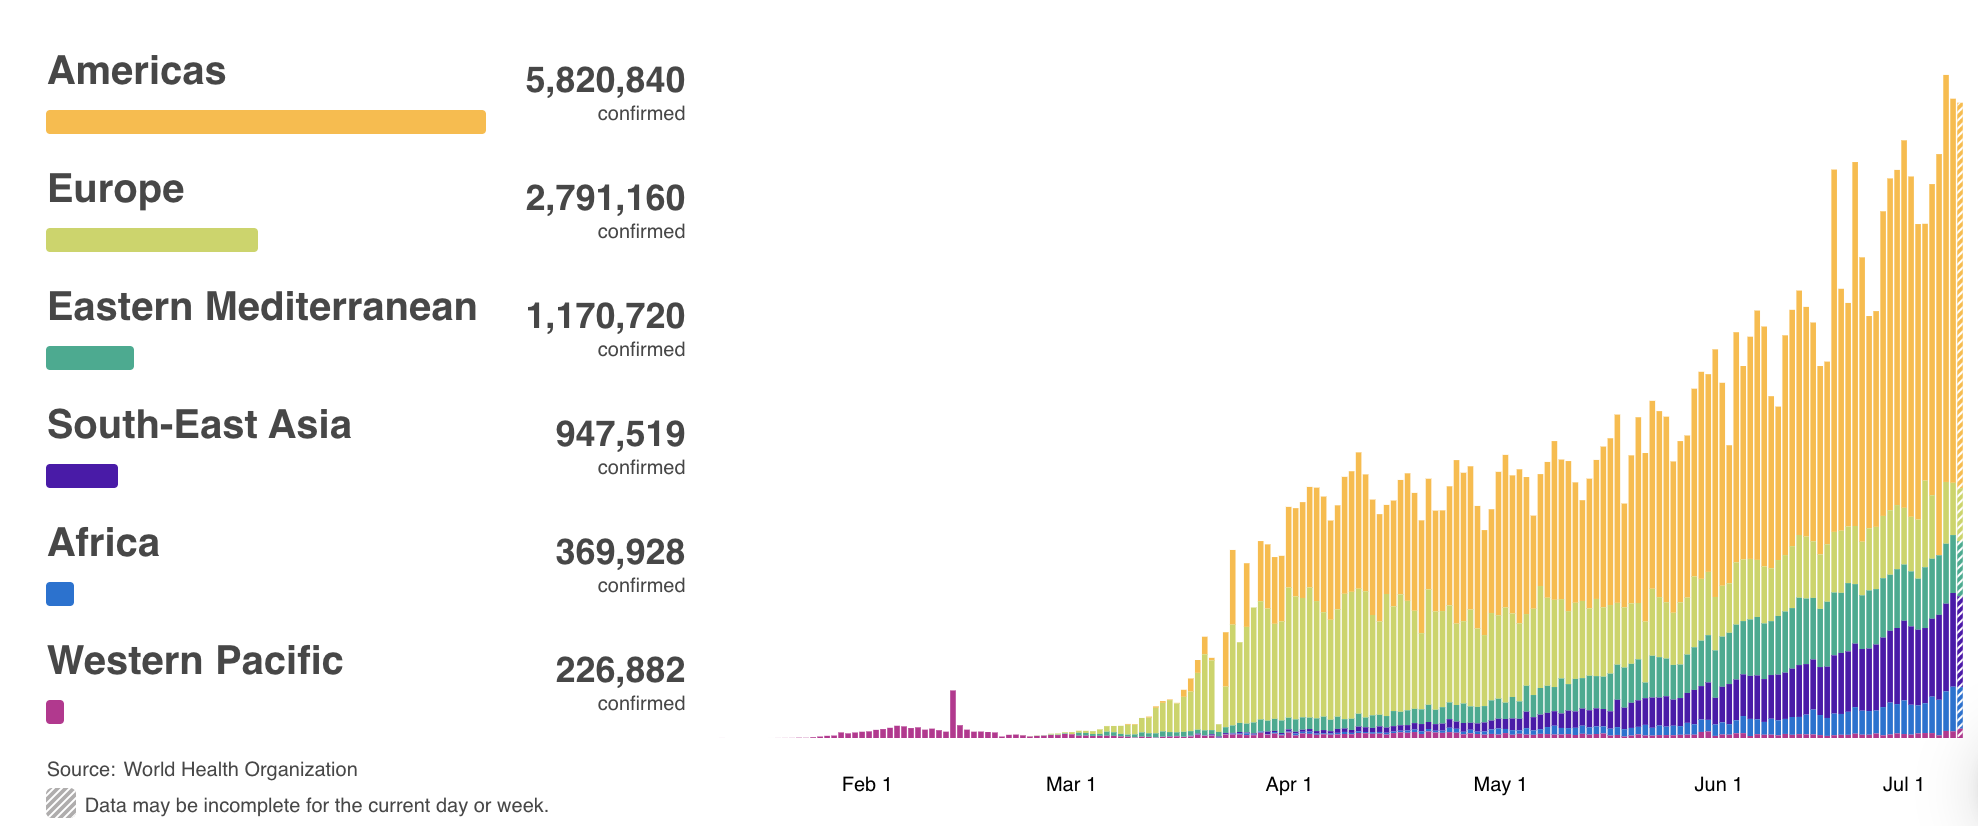
\includegraphics[]{./input/covid1.png} %插入图片,[]中设置图片大小,{}中是图片文件名
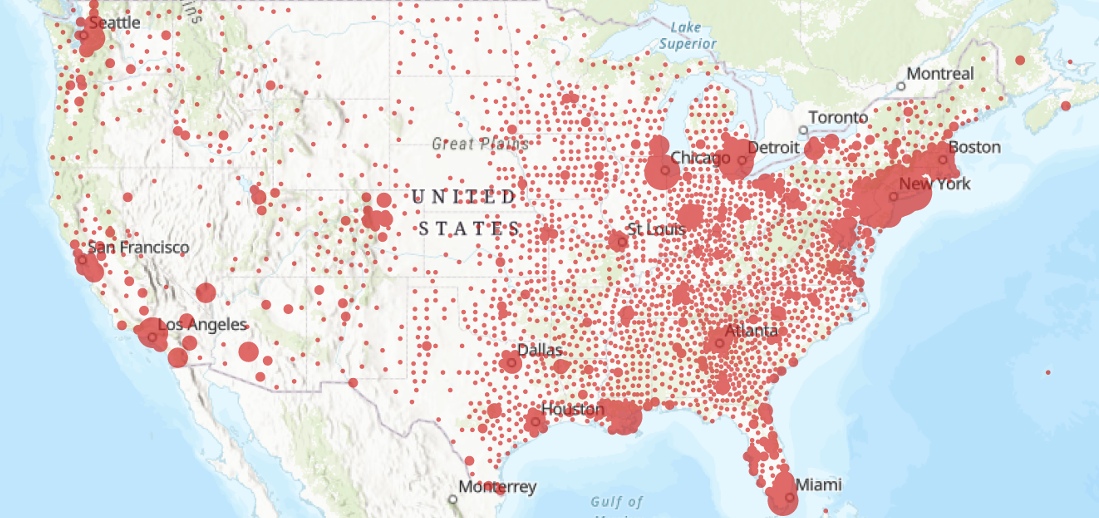
\includegraphics[]{./input/covid4.png}
\label{} %用于文内引用的标签
\end{figure}

\begin{table}[H]
    \centering \begin{table}[H]
\centering\begingroup\fontsize{20}{22}\selectfont

\resizebox{\linewidth}{!}{
\begin{tabular}{rlrrrr}
\toprule
\multicolumn{0}{c}{\textbf{ }} & \multicolumn{5}{c}{\textbf{表1 累计确诊前十位国家}} \\
  & 国家(地区) & 累计确诊 & 粗发病率* & 累计死亡 & 病死率\%\\
\midrule
\rowcolor{gray!6}  1 & 美国 US & 3,363,056 & 1,016 & 135,605 & 4.0\\
2 & 巴西 Brazil & 1,884,967 & 887 & 72,833 & 3.9\\
\rowcolor{gray!6}  3 & 印度 India & 906,752 & 66 & 23,727 & 2.6\\
4 & 俄罗斯 Russia & 732,547 & 502 & 11,422 & 1.6\\
\rowcolor{gray!6}  5 & 秘鲁 Peru & 330,123 & 1,001 & 12,054 & 3.7\\
6 & 智利 Chile & 317,657 & 1,662 & 7,024 & 2.2\\
\rowcolor{gray!6}  7 & 墨西哥 Mexico & 304,435 & 236 & 35,491 & 11.7\\
8 & 英国 UK & 291,691 & 430 & 44,915 & 15.4\\
\rowcolor{gray!6}  9 & 南非 South Africa & 287,796 & 485 & 4,172 & 1.4\\
10 & 伊朗 Iran & 259,652 & 309 & 13,032 & 5.0\\
\bottomrule
\end{tabular}}
\endgroup{}
\end{table} \begin{tablenotes}
        \fontsize{12}{12}
        \selectfont
        \item 注:*粗发病率定义:在一定时间内,特定范围人群中某病新发生的病例出现的频率。计算方式:(累计确诊病例/人口)×10万;
      \end{tablenotes}
    \end{table}

\begin{table}[H]
    \centering \begin{table}[H]
\centering\begingroup\fontsize{20}{22}\selectfont

\begin{tabular}{rlrr}
\toprule
\multicolumn{0}{c}{\textbf{ }} & \multicolumn{2}{c}{\textbf{表2 日新增病例前十位国家}} \\
  & 国家 & 新增确诊 & 新增死亡\\
\midrule
\rowcolor{gray!6}  1 & 美国 US & 58,114 & 400\\
2 & 印度 India & 28,498 & 553\\
\rowcolor{gray!6}  3 & 巴西 Brazil & 20,286 & 733\\
4 & 南非 South Africa & 11,554 & 93\\
\rowcolor{gray!6}  5 & 俄罗斯 Russia & 6,511 & 104\\
6 & 哥伦比亚 Colombia & 5,083 & 208\\
\rowcolor{gray!6}  7 & 墨西哥 Mexico & 4,685 & 485\\
8 & 秘鲁 Peru & 3,797 & 184\\
\rowcolor{gray!6}  9 & 哈萨克斯坦 Kazakhstan & 3,502 & 0\\
10 & 阿根廷 Argentina & 3,099 & 58\\
\bottomrule
\end{tabular}
\endgroup{}
\end{table} \end{table}
\vspace{5mm}
\begin{minipage}{\textwidth}
  \begin{figure}[H]
  \centering
  \captionsetup{font={huge}}
  \caption{日新增确诊病例前五位国家趋势图}
  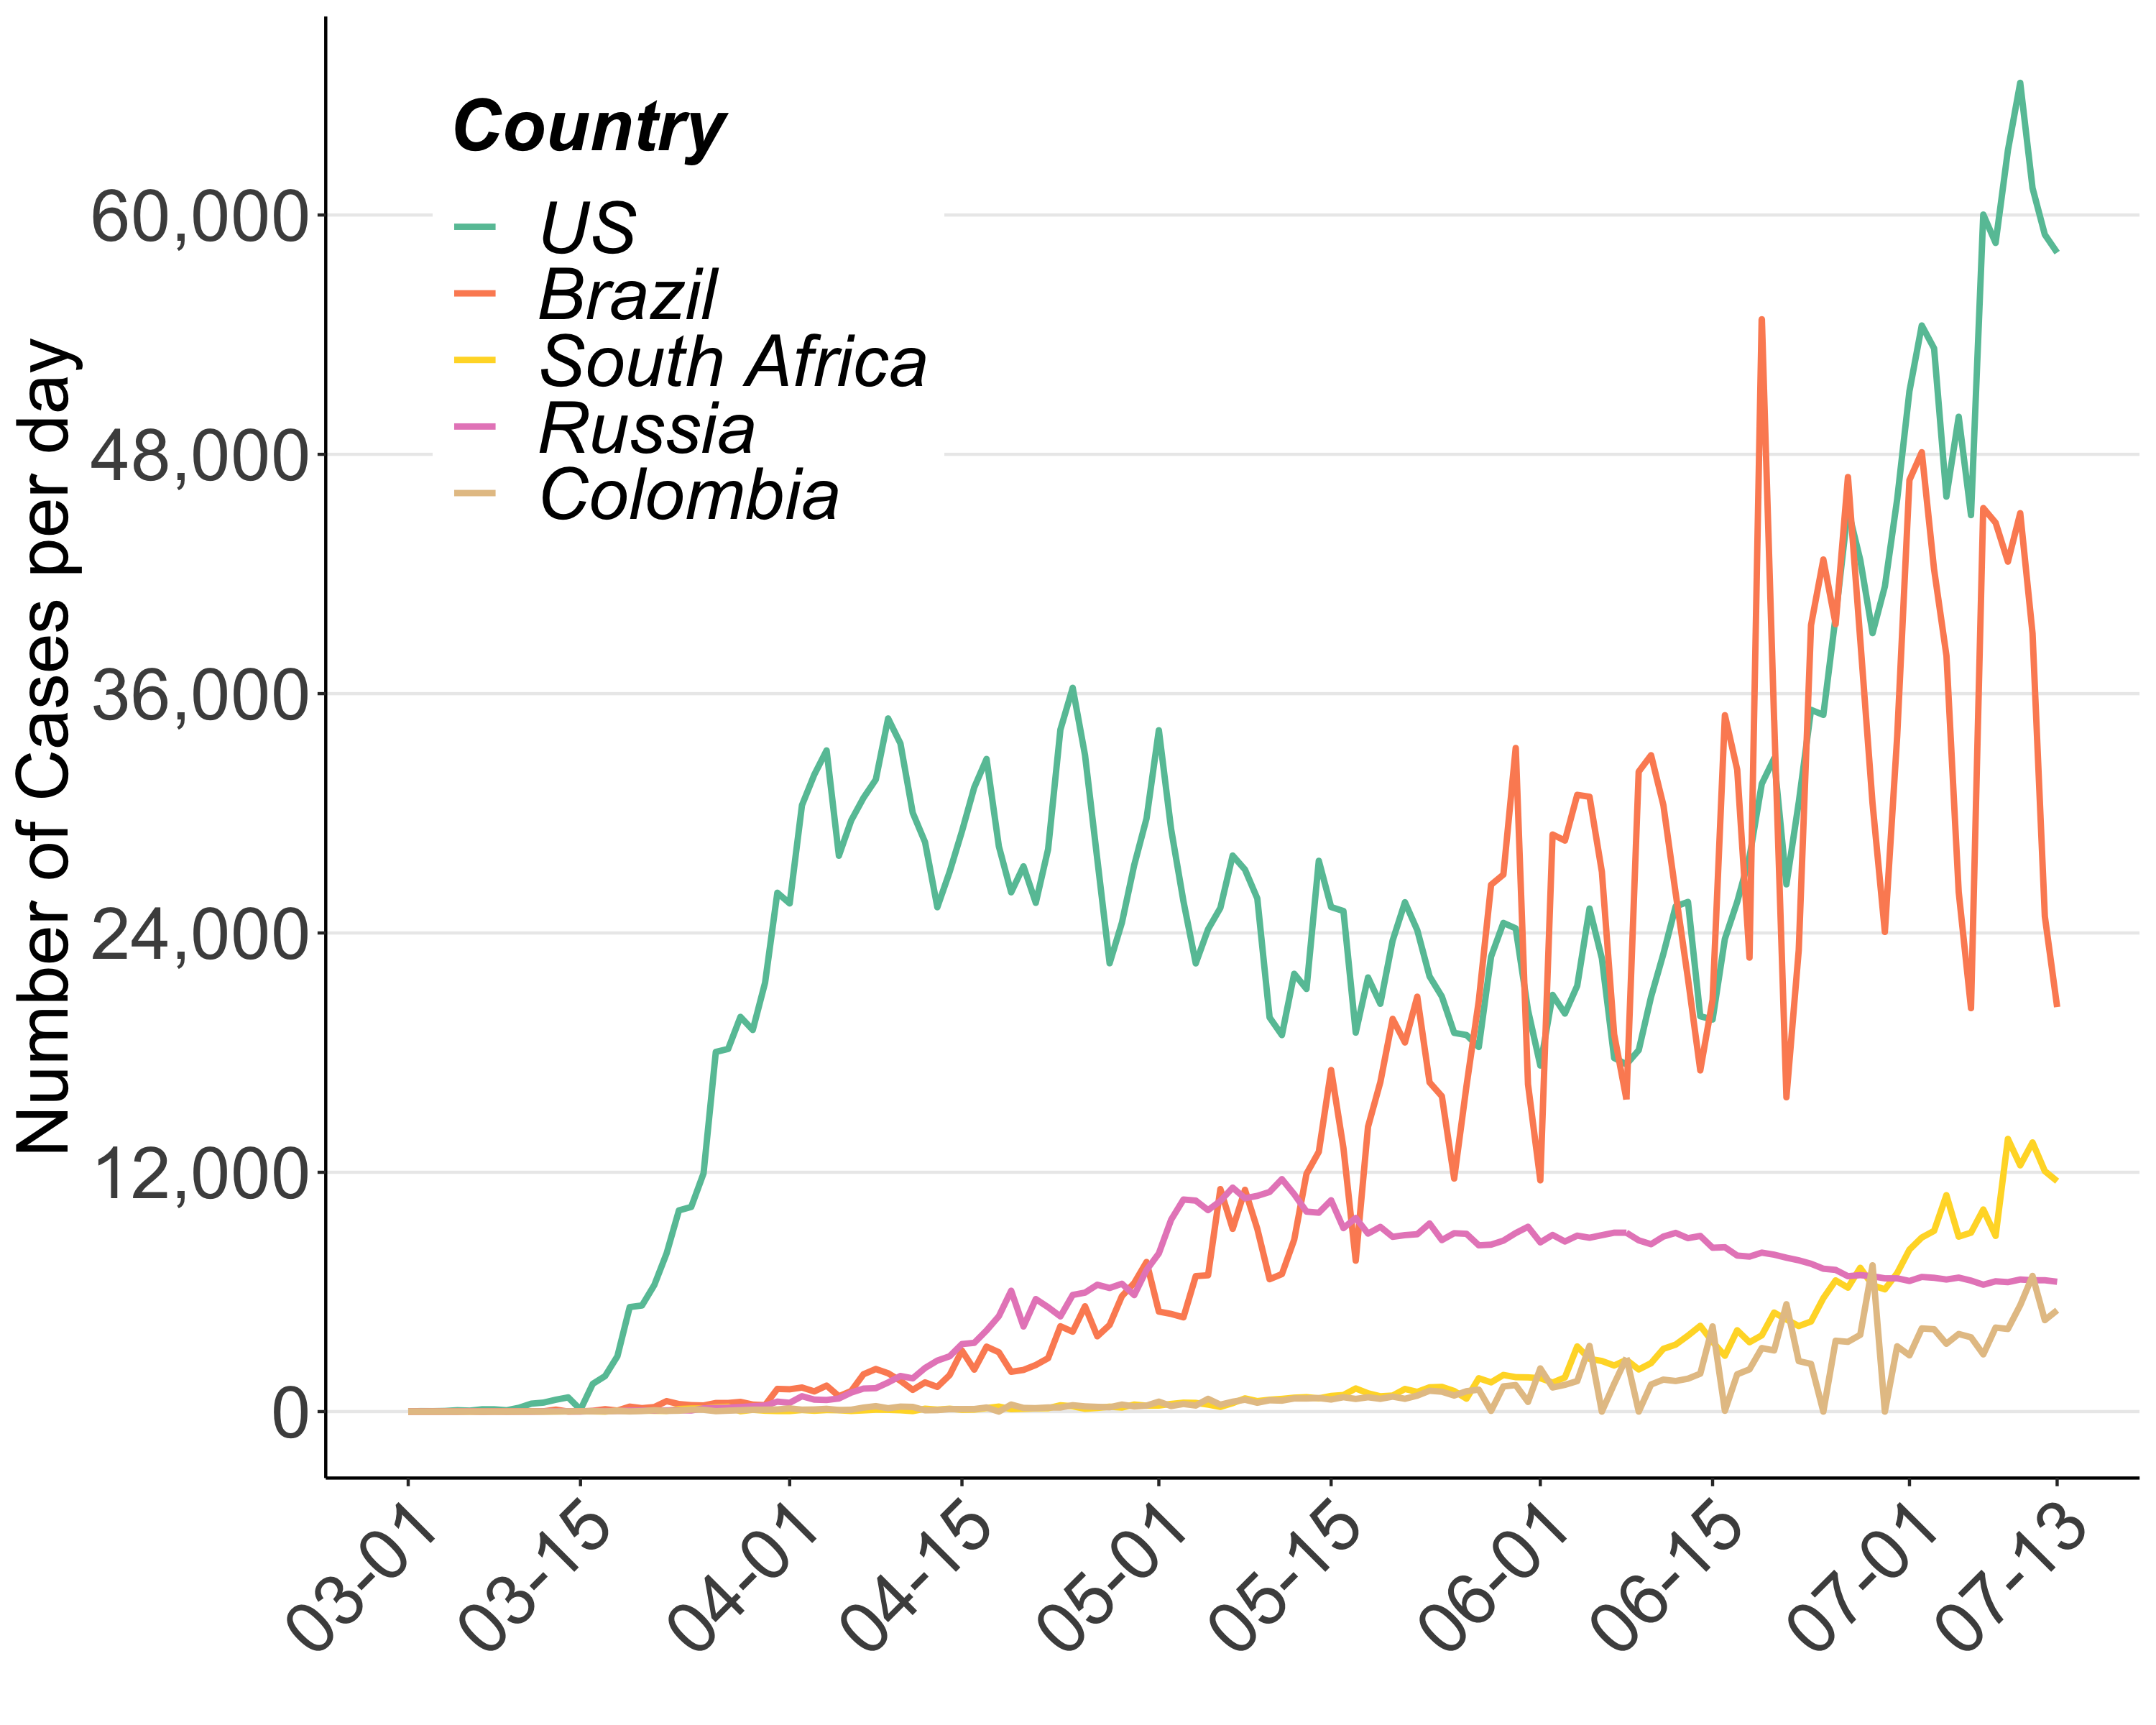
\includegraphics[]{./input/covid2.png}
  \captionsetup{font=large}\caption*{注:图中显示为7日移动平均值,计算方式(当天+前6天)/7。}
  \end{figure}
\end{minipage}

\begin{minipage}{\textwidth}
  \begin{figure}[H]
  \centering
  \captionsetup{font={huge}}
  \caption{日新增死亡病例前五位国家趋势图}
  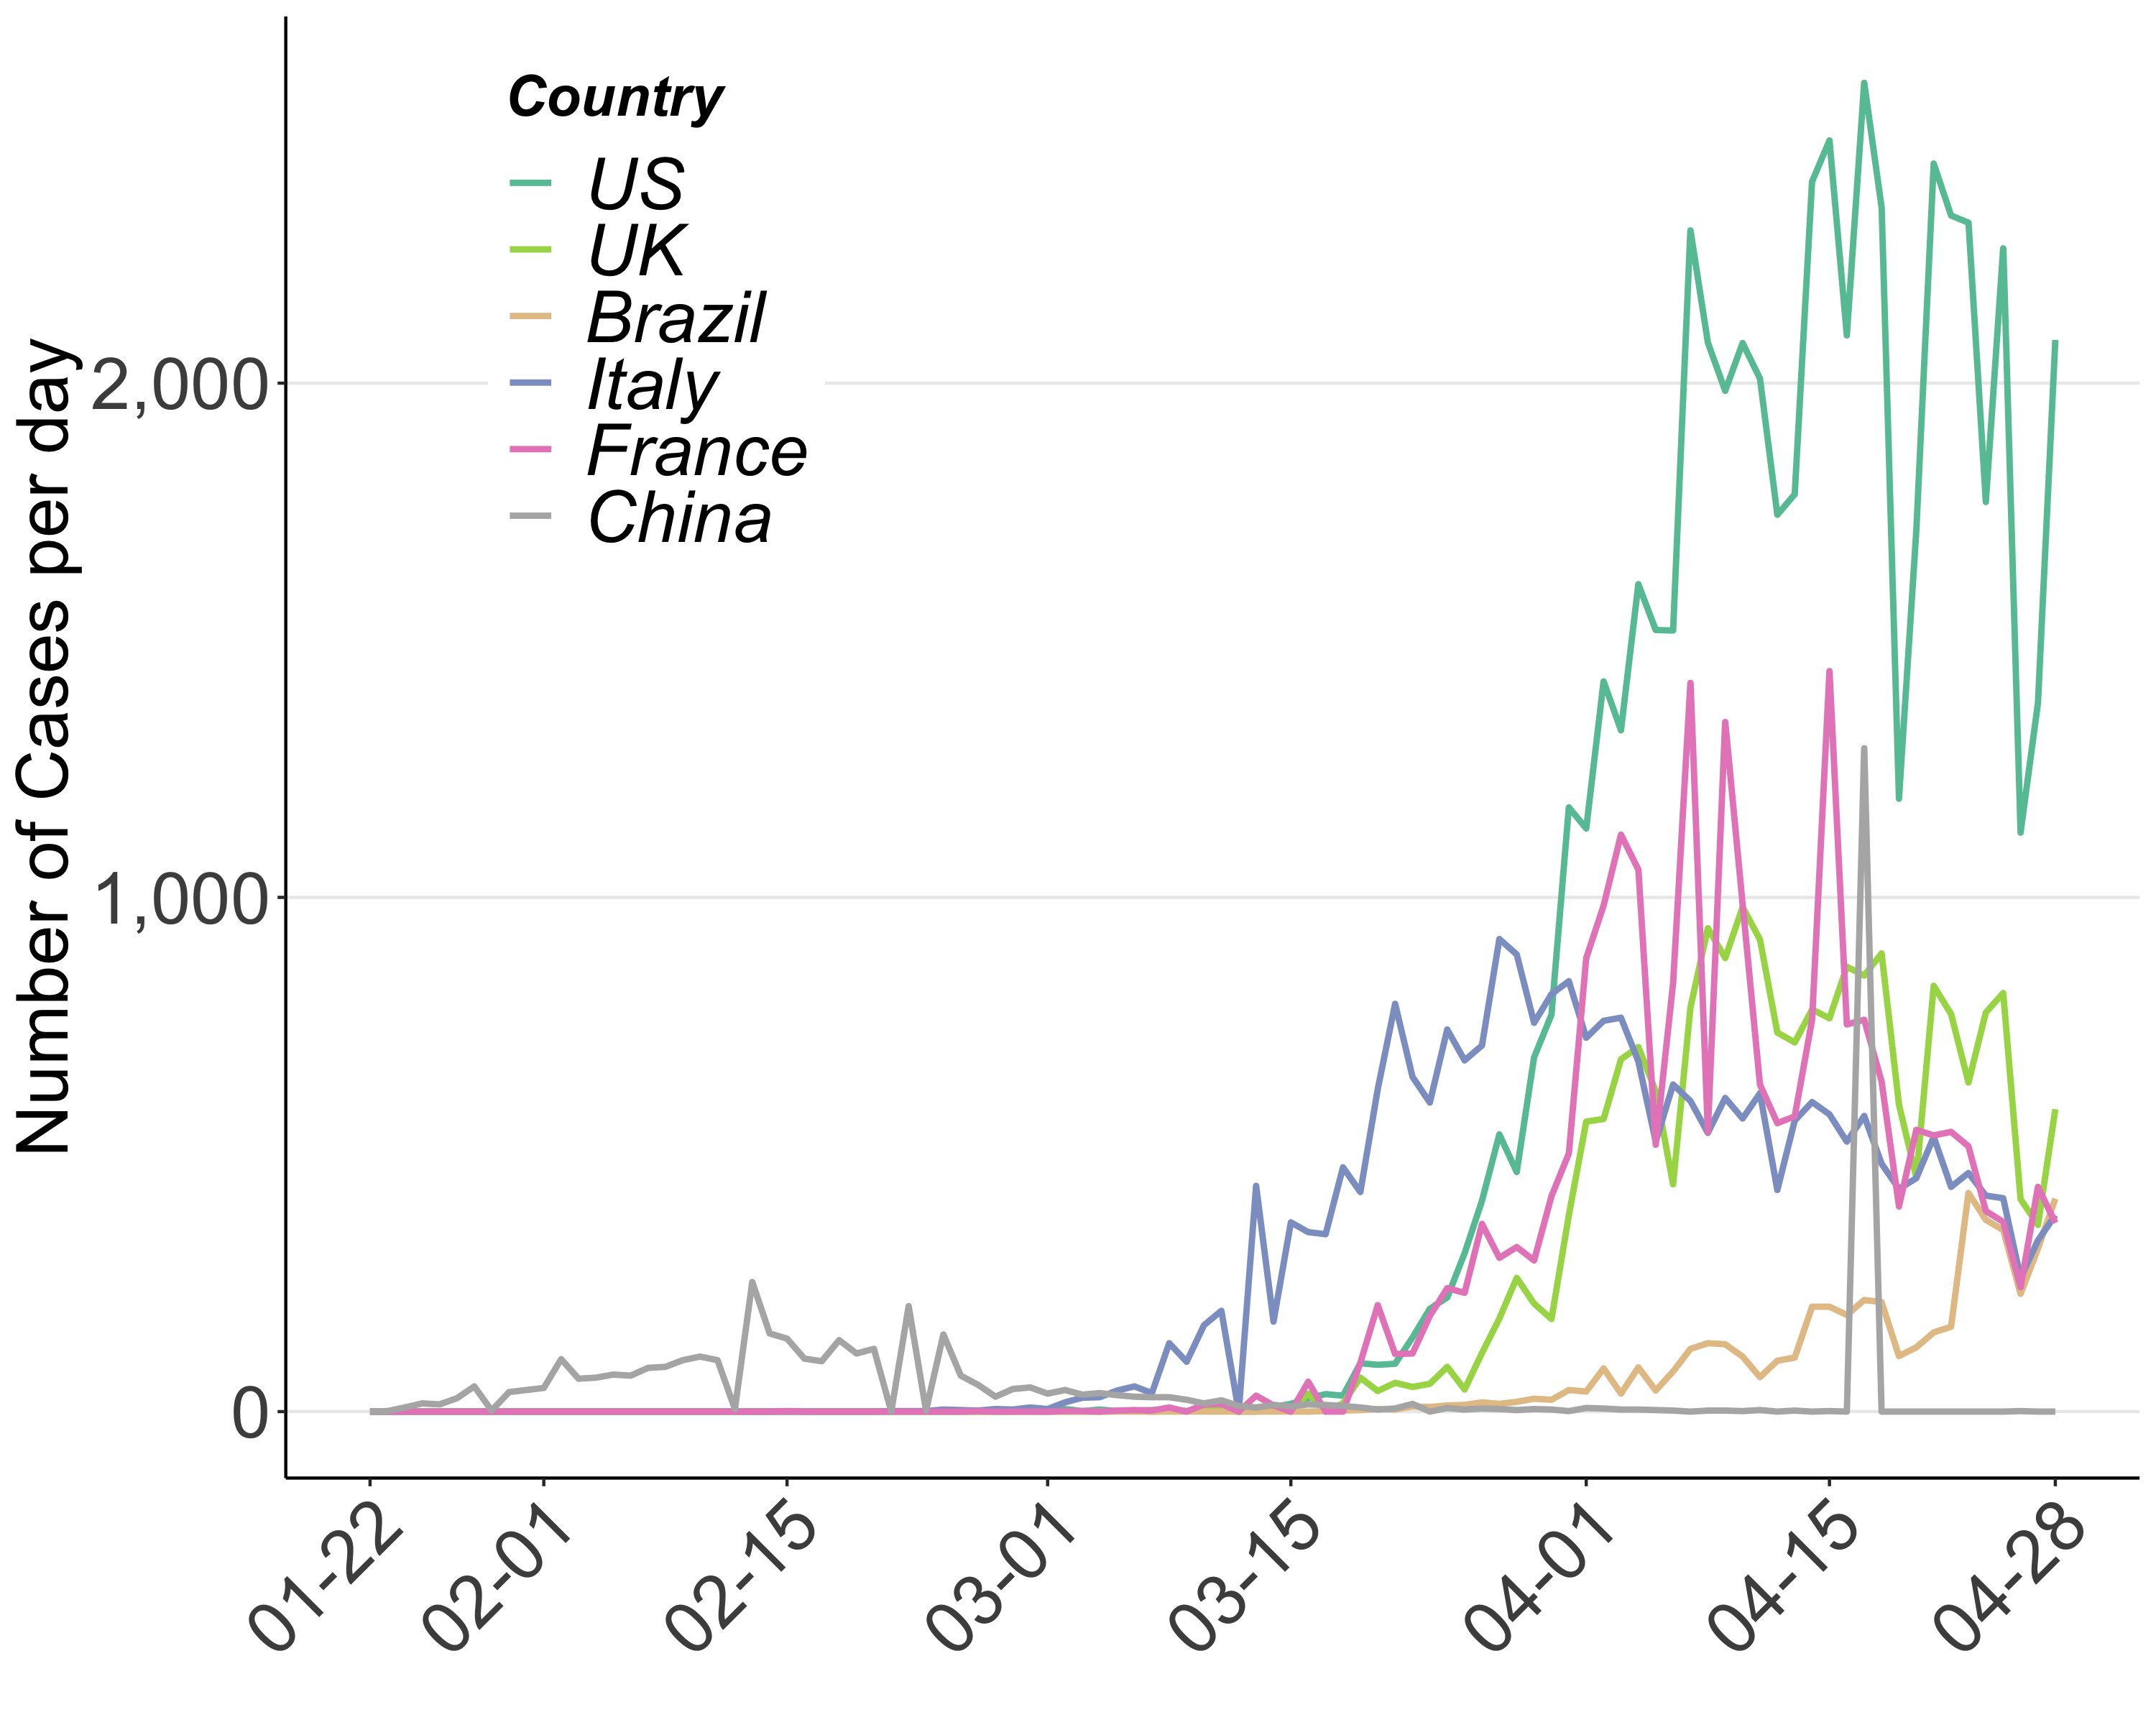
\includegraphics[]{./input/covid3.png}
  \captionsetup{font=large}\caption*{注:图中显示为7日移动平均值,计算方式(当天+前6天)/7。}
  \end{figure}
\end{minipage}

\begin{huge}{\textcolor{glaucous}{\textbf {二、美国疫情}}}\end{huge}

\begin{minipage}{\textwidth}
  \begin{figure}[H]
  \centering
  \captionsetup{font={huge}}
  \caption{美国日新增确诊前五位州趋势图}
  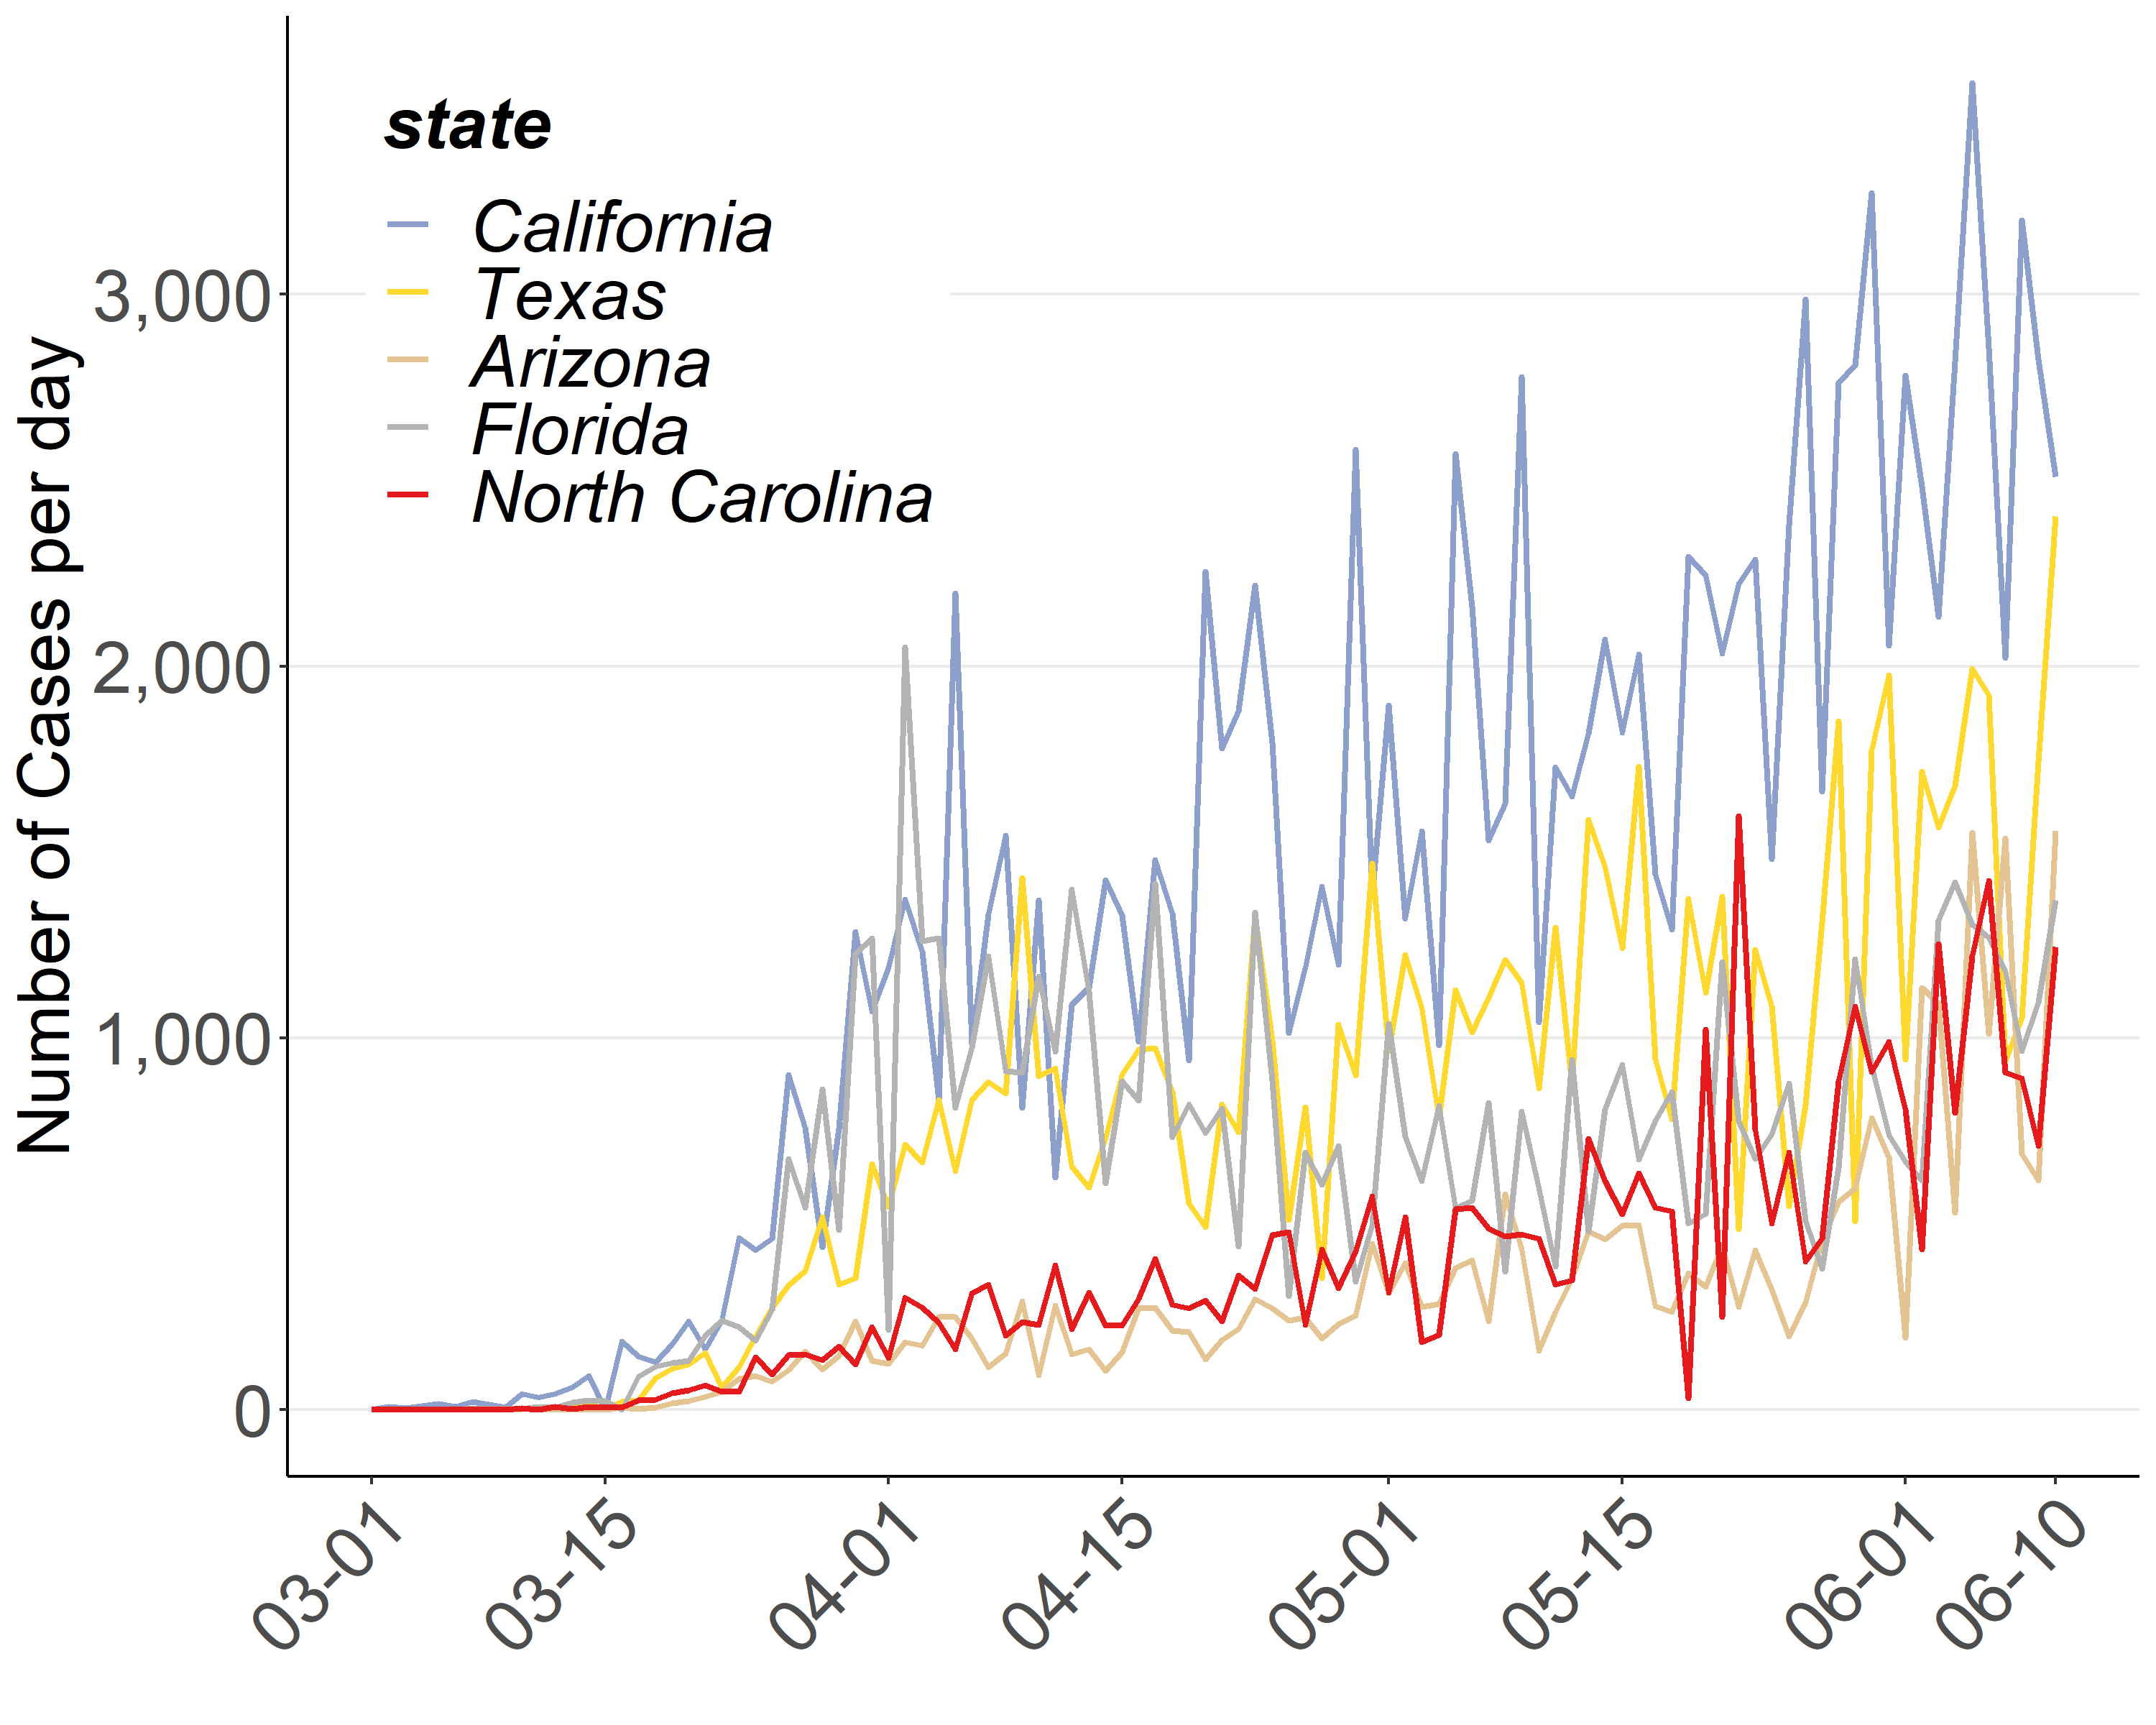
\includegraphics[]{./input/covid5.png}
  \captionsetup{font=large}\caption*{注:图中显示为7日移动平均值,计算方式(当天+前6天)/7。}
  \end{figure}
\end{minipage}

\begin{minipage}{\textwidth}
  \begin{figure}[H]
  \centering
  \captionsetup{font={huge}}
  \caption{美国日新增死亡前五位州趋势图}
  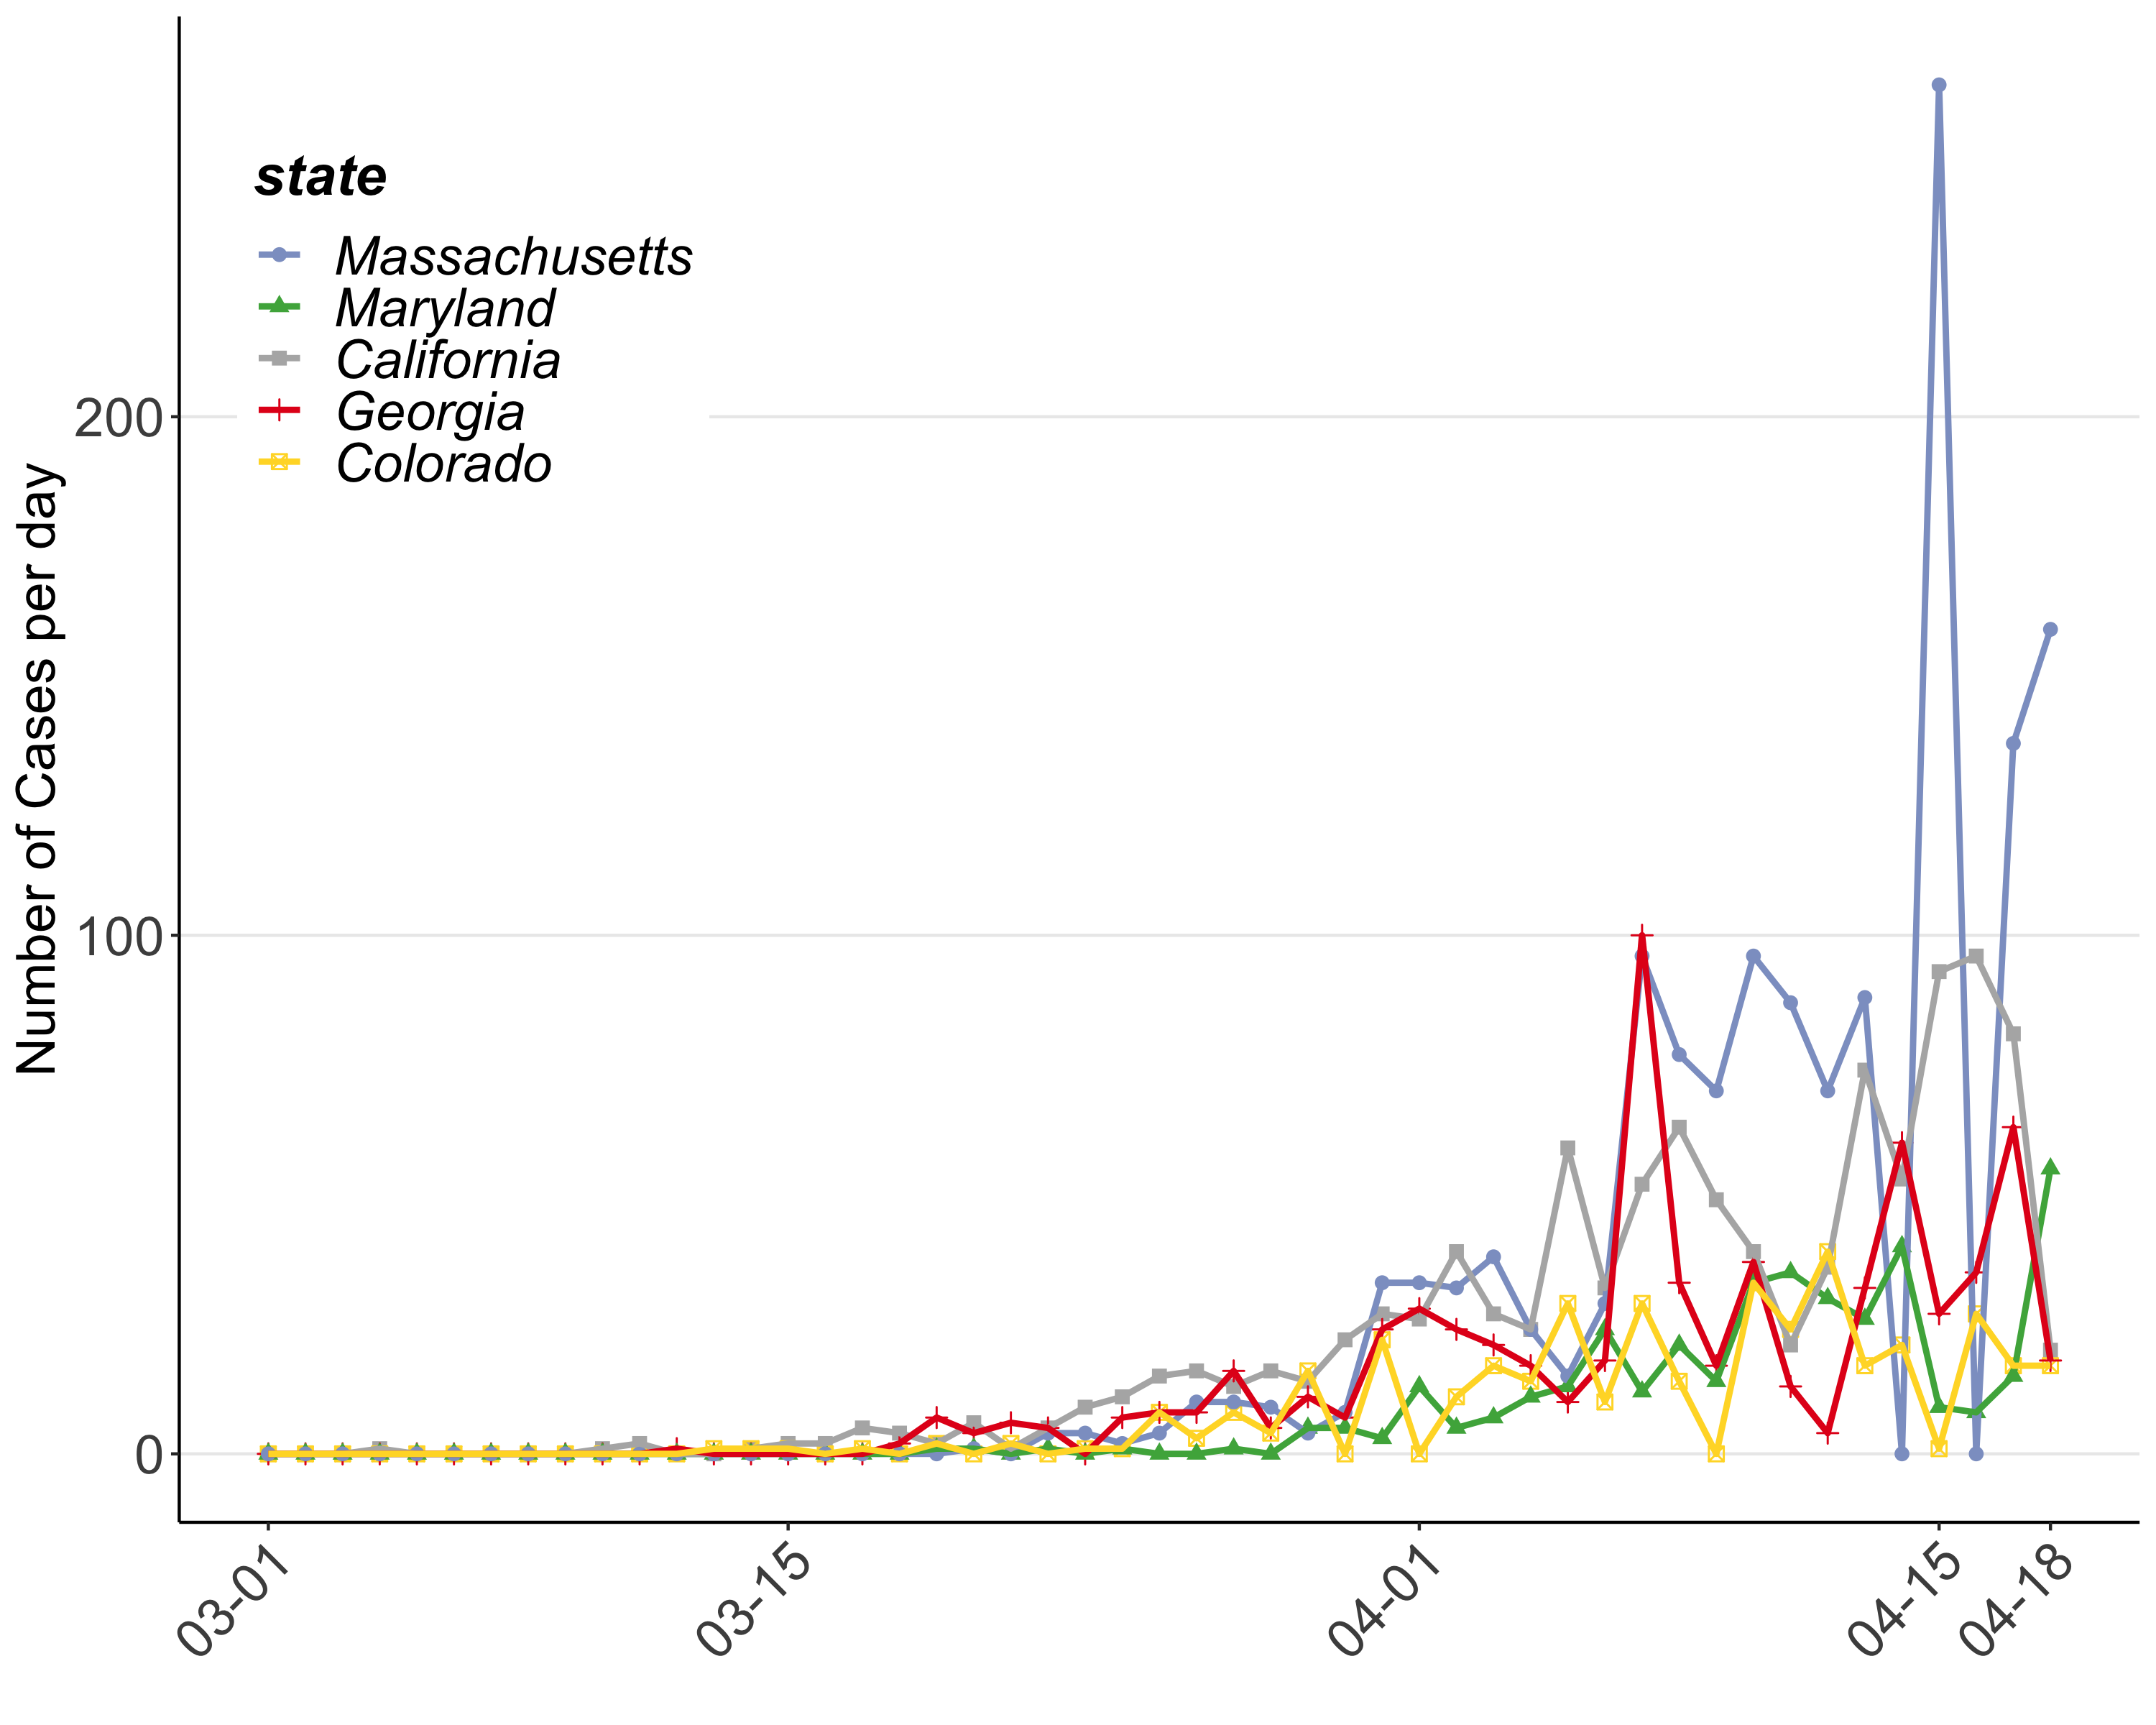
\includegraphics[]{./input/covid6.png}
  \captionsetup{font=large}\caption*{注:图中显示为7日移动平均值,计算方式(当天+前6天)/7。}
  \end{figure}
\end{minipage}

\begin{table}[H]
    \centering \begin{table}[H]
\centering\begingroup\fontsize{20}{22}\selectfont

\resizebox{\linewidth}{!}{
\begin{tabular}{rlrr}
\toprule
\multicolumn{0}{c}{\textbf{ }} & \multicolumn{3}{c}{\textbf{表3 美国新增确诊前十位州}} \\
  & 国家/州名 & 当日新增 & 累计确诊\\
\midrule
\rowcolor{gray!6}   & 美国 US & 58,114 & 3,363,056\\
1 & 佛罗里达州 FL & 12,624 & 282,435\\
\rowcolor{gray!6}  2 & 加利福尼亚州 CA & 8,814 & 333,357\\
3 & 得克萨斯州 TX & 7,016 & 269,778\\
\rowcolor{gray!6}  4 & 乔治亚州 GA & 3,637 & 120,572\\
5 & 田纳西州 TN & 3,314 & 65,274\\
\rowcolor{gray!6}  6 & 阿拉巴马州 AL & 1,958 & 55,545\\
7 & 北卡罗莱纳州 NC & 1,898 & 87,669\\
\rowcolor{gray!6}  8 & 路易斯安那州 LA & 1,705 & 79,827\\
9 & 南卡罗来纳州 SC & 1,520 & 58,168\\
\rowcolor{gray!6}  10 & 亚利桑那州 AZ & 1,357 & 123,824\\
\bottomrule
\end{tabular}}
\endgroup{}
\end{table} \end{table}\begin{table}[H]
    \centering \begin{table}[H]
\centering\begingroup\fontsize{20}{22}\selectfont

\resizebox{\linewidth}{!}{
\begin{tabular}{rlrrr}
\toprule
\multicolumn{0}{c}{\textbf{ }} & \multicolumn{4}{c}{\textbf{表4 美国新增死亡前十位州}} \\
  & 国家/州名 & 当日新增 & 累计死亡 & 病死率\%\\
\midrule
\rowcolor{gray!6}   & 美国 US & 400 & 135,605 & 4.0\\
1 & 得克萨斯州 TX & 60 & 3,276 & 1.2\\
\rowcolor{gray!6}  2 & 纽约州 NY & 45 & 32,395 & 8.1\\
3 & 加利福尼亚州 CA & 38 & 7,089 & 2.1\\
\rowcolor{gray!6}  4 & 佛罗里达州 FL & 35 & 4,277 & 1.5\\
5 & 新泽西州 NJ & 35 & 15,560 & 8.9\\
\rowcolor{gray!6}  6 & 康涅狄格州 CT & 23 & 4,371 & 9.2\\
7 & 乔治亚州 GA & 23 & 3,026 & 2.5\\
\rowcolor{gray!6}  8 & 密苏里州 MO & 13 & 1,105 & 3.9\\
9 & 南卡罗来纳州 SC & 11 & 972 & 1.7\\
\rowcolor{gray!6}  10 & 亚利桑那州 AZ & 9 & 2,246 & 1.8\\
\bottomrule
\end{tabular}}
\endgroup{}
\end{table} \begin{tablenotes}
        \fontsize{15}{15}
        \selectfont
        \item
      \end{tablenotes}
\end{table}

\vspace{5mm}

\centering
\fontsize{12}{12}
\selectfont
\begin{tabular}{ll}


主编:马晶  &  副主编:仁晖\, 史珂玮\, 霍舒同 \\
责任编辑: 曹洁  \\
新闻组:闫怡璇\, 吴舒兰 &  数据分析:徐蕴汶 \\
热点话题:李祎杰 & 微信排版:韩佩瑾\, 李萱\, 王艺晓\\
\multicolumn{2}{l}{可视化组:周梓淇\, 刘逸洋\, 唐星鸿\, 曹洁\, 孙昊\, 张立达}

\end{tabular}

\end{document}
